\documentclass[aspectratio=169]{beamer}
\geometry{paperwidth=160mm,paperheight=100mm}
\usepackage{beamerthemesidebar}
\usepackage{hyperref}
\usepackage{color}
\usepackage{multimedia}
\usepackage{colortbl}
\usepackage{amsmath}
\usepackage{empheq}
\usepackage{cancel}
\usepackage{amssymb}
\usepackage{amsfonts}
\usepackage{lipsum}
\usepackage{tcolorbox}
\usepackage{tabularx}
\usepackage{caption}
\usepackage{bm}

\setbeamersize{sidebar width right=0pt}
\setbeamertemplate{footline}[frame number]
%
\definecolor{orange}{RGB}{250,167,12}
\definecolor{yellow}{RGB}{246,250,12}
\definecolor{green}{RGB}{128,238,1}
\definecolor{black}{RGB}{0,0,0}
\definecolor{blue}{RGB}{0,0,255}
\definecolor{red}{RGB}{255,0,0}
\definecolor{sepia}{RGB}{94,38,18}
\newcommand{\ve}[1]{{\rm\bf {#1}}}
\newcommand{\q}[1]{\textcolor{blue}{#1}}
\newcommand{\blue}[1]{\textcolor{blue}{#1}}
\newcommand{\sepia}[1]{\textcolor{sepia}{#1}}
\newcommand{\red}[1]{\textcolor{red}{#1}}
\newcommand{\green}[1]{\textcolor{green}{#1}}
\newcommand{\yellow}[1]{\textcolor{yellow}{#1}}
\newcommand{\orange}[1]{\textcolor{orange}{#1}}
\definecolor{burlywood}{RGB}{255,211,155}
\definecolor{chocolate}{RGB}{255,127,36}
\definecolor{tan}{RGB}{210,180,140}
%
\def\onethird{{\textstyle{1\over3}}}
\def\twothirds{{\textstyle{2\over3}}}
\def\fourthirds{{\textstyle{4\over3}}}
\def\onehalf{{\textstyle{1\over2}}}
\def\threehalfs{{\textstyle{3\over2}}}
%
\newcommand{\pd}{\partial}
\newcommand{\aMLT}{\alpha_{\rm MLT}}
\newcommand{\Fconv}{F_{\rm conv}}
\newcommand{\Frad}{F_{\rm rad}}
\newcommand{\Ftot}{F_{\rm tot}}
\newcommand{\Hp}{H_p}
\newcommand{\prad}{p_{\rm rad}}
\newcommand{\pgas}{p_{\rm gas}}
\newcommand{\TTc}{T_{\rm c}}
\newcommand{\rhoc}{\rho_{\rm c}}
\newcommand{\Teff}{T_{\rm eff}}
\newcommand{\Fstar}{F_\star}
\newcommand{\pstar}{p_\star}
\newcommand{\Pstar}{P_\star}
\newcommand{\Rstar}{R_\star}
\newcommand{\rhostar}{\rho_\star}
\newcommand{\Tstar}{T_\star}
%
\title{Theoretical Astrophysics I: Physics of Sun and Stars\\
Lecture 7: Simple Overview of Stellar Evolution}
\author{\texorpdfstring{\sepia{Petri K\"{a}pyl\"{a} Ivan Mili\'{c}}\newline\blue{\url{pkapyla, milic@leibniz-kis.de}}}{}}
\institute{Institut f\"ur Sonnenphysik - KIS, Freiburg}
\date{\today}
%
\begin{document}
\frame{\titlepage}

% Characterization of the logT logrho lane
% Evolution of a star as viewed from the centre
% Theory of the main sequence
% Structure of stars in late evolutionary stages
% Shortcomings of the simple picture

% - Core of the star determines the stellar evolution, outer regions follow
% - As fuel in core is depleted, evolution progresses
% - Following just the core gives an idea of evolution of stars (=simple picture)

% - Temperature, density and composition determine all other properties
% - Follow T_c(t), \rho_c(t), stellar evolution is described by a succession 
%   of core values at different times t_1, t_2, t_3, etc...
% - For the same composition, the mass determines the rest

% - Combinations of T and \rho determine which physical processes are at work
% - This leads to a "terrain" where the star evolves as T and \rho change
% - The terrain consists of zones dominated by different equations of state and
%   nuclear processes
% - In some conditions dynamical instabilities may occur which are of specific
%   interest

% - Show Fig. 7.1 and explain the regimes of different equations of state

% - Nuclear reaction regimes (given nuclear process becomes important when a
%   sizeable fraction of stellar luminosity if produced by it)
% - Luminosity varies immensely, but nuclear reactions are much more restricted
%   because of their strong T-dependence. This leads to a sharp threshold.

% - Dynamical stability (6.3)
% - \gamma_a > 4/3 (cool outer layers of stars, but not relevant for global
%   stability)
% - Strict bounds in terms of density and temperature: severe constraints for
%   evolutionary tracks of stars

% - Can a star obtain any values of T_c, \rho_c or is this constrained by M?
% - Use polytropic eos to describe the central density (good approximation
%   regardless why gas is polytopic)
% - Star of fixed mass has a distinct track in the T_c,\rho_c plane.

% - Qualitatively different paths of massive and light stars!

% - Explain degeneracy!
% - Chandrasekhar mass
% - White dwarfs: larger mass => lower radius

% - Degenerate gas thermally unstable: carbon burning leads to thermonuclear runaway
%   (supernovae in close binaries)

% - Stars above M_Ch: unstable iron-photondisintegration boundary (supernovae)
% - Very massive stars: pair production instability => explosion at a young age

% - Homology relations
% - Homogeneity is the main weakness of the homology relations

% - Explain the red giant / supergiant phase


\section{Evolution of stars - schematic picture}
%
\frame{
\frametitle{The ($T,\rho$)-plane}
\begin{itemize}
\item The evolution of the star is driven by its core. \blue{Why?}
\item If we know the chemical composition, density $\rho$, and the
  temperature $T$, all other quantities can be derived.
\item Let us denote the pair of central temperature and density at
  time $t$ as $[\TTc(t),\rhoc(t)]$.
\item Then the evolution of the star is described by a succession of
  states $[\TTc(t_1),\rhoc(t_1)]$, $[\TTc(t_2),\rhoc(t_2)]$,
  $[\TTc(t_3),\rhoc(t_3)]$, $\ldots$, at times $t_1$, $t_2$, $t_3$,
  $\ldots$, forming a parametric line $[\TTc(t),\rhoc(t)]$.
\item Assuming stars with the same composition, we expect that the
  $[\TTc(t),\rhoc(t)]$ depend on stellar mass $M$.
\end{itemize}
}
%
\frame{
\frametitle{Characterization of the ($\log T,\log\rho$)-plane}
\begin{itemize}
\item We anticipate that $T$ and $\rho$ can vary several orders of
  magnitude depending on the star and/or evolutionary stage, we
  consider the logarithms $\log T$ and $\log\rho$ in what follows.
\item The ($\log T,\log\rho$)-plane divides into zones where different
  equations of state, nuclear reactions, and dynamical instabilities
  dominate.
\item We begin with the equations of state. The most common state is
  described by the ideal gas equation:
  \begin{equation}
    p_{\rm ideal} = \frac{{\cal R}}{\mu} \rho T = K_0 \rho T,
  \end{equation}
  where $K_0$ is a constant. At high density (and not too high
  temperature), the electrons become degenerate and dominate the
  pressure according to
  \begin{equation}
    p_{\rm e,deg} = K_1 \rho^{5/3},
  \end{equation}
  where $K_1$ is another constant.
  \end{itemize}
}
%
\frame{
\frametitle{Characterization of the ($\log T,\log\rho$)-plane}
\begin{minipage}{0.5\linewidth}
\begin{itemize}
\item The border between these lies along a line where $p_{\rm ideal}
  = p_{\rm e,deg}$, or
  \begin{equation}
    \log\rho = 1.5 \log T + {\rm const.}
  \end{equation}
  This line separates regions I and II.
\item For relativistic degeneracy %the gas pressure is
  \begin{equation}
    p_{\rm e,r-deg} = K_1 \rho^{4/3},\label{equ:perdeg}
  \end{equation}
  corresponding to 
  \begin{equation}
    \log\rho = 3 \log T + {\rm const.}
  \end{equation}
  w.r.t. ideal gas separating regions I and III.
\end{itemize}
\end{minipage}
\begin{minipage}{0.49\linewidth}
\begin{figure}
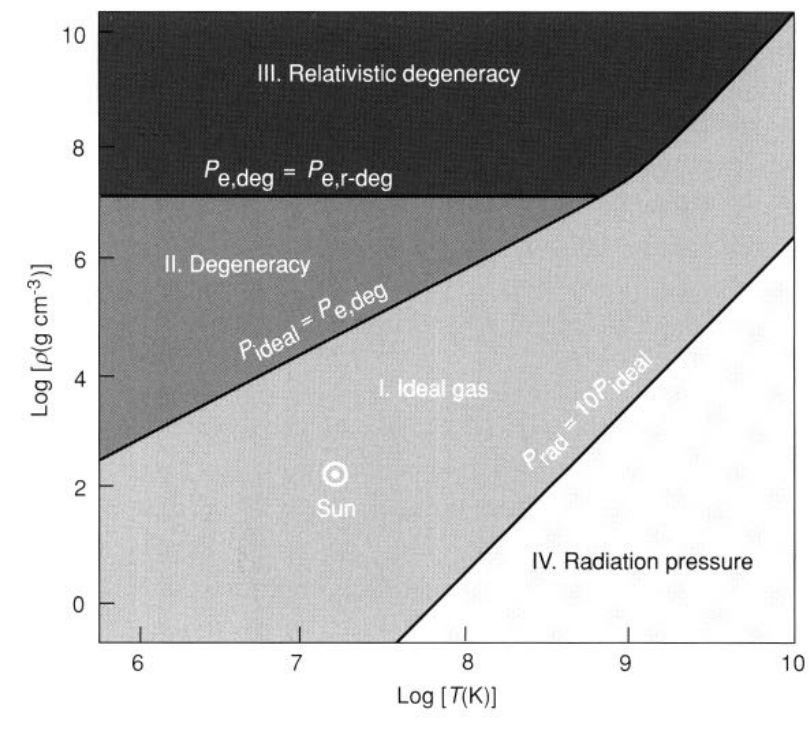
\includegraphics[width=6.5cm]{figures//Prialnik_logTlogrho_eos.png}
\caption*{Credits: Prialnik}
\end{figure}
\end{minipage}
}
%
%
\frame{
\frametitle{Characterization of the ($\log T,\log\rho$)-plane}
\begin{minipage}{0.5\linewidth}
\begin{itemize}
\item Transition from standard to relativistic degeneracy occurs for
  $\rho \gg (K_2/K_1)^3$ (regions II and III).
\item For sufficiently low pressure and high temperature the radiation
  pressure with
  \begin{equation}
    p = \onethird a T^4,
  \end{equation}
  becomes dominant. This again leads to:
  \begin{equation}
    \log\rho = 3 \log T + {\rm const.}
  \end{equation}
  separating regions I and IV.
\end{itemize}
\end{minipage}
\begin{minipage}{0.49\linewidth}
\begin{figure}
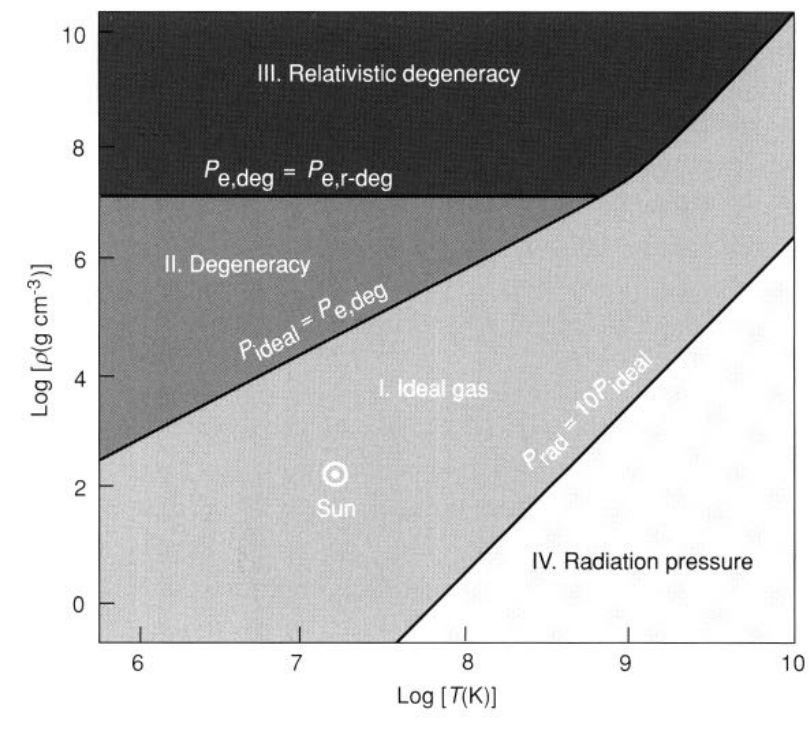
\includegraphics[width=6.5cm]{figures//Prialnik_logTlogrho_eos.png}
\caption*{Credits: Prialnik}
\end{figure}
\end{minipage}
}
%
%
\frame{
\frametitle{Zones of nuclear burning}
\begin{minipage}{0.5\linewidth}
\begin{itemize}
\item Nuclear energy generation can be approximated by a power law
  \begin{equation}
    q = q_0 \rho^m T^n.
  \end{equation}
\item A given reaction becomes important when $q>q_{\rm min}$
  (e.g.~0.1~J~km$^{-1}$~s$^{-1}$). This leads to
  \begin{equation}
    \log\rho = - \frac{n}{m}\log T + \frac{1}{m} \log \left(
    \frac{q_{\rm min}}{q_0} \right).
  \end{equation}
\item For most reactions $n\gg m$ so the temperature determines the
  ignition of nuclear reactions.
\end{itemize}
\end{minipage}
\begin{minipage}{0.49\linewidth}
\begin{figure}
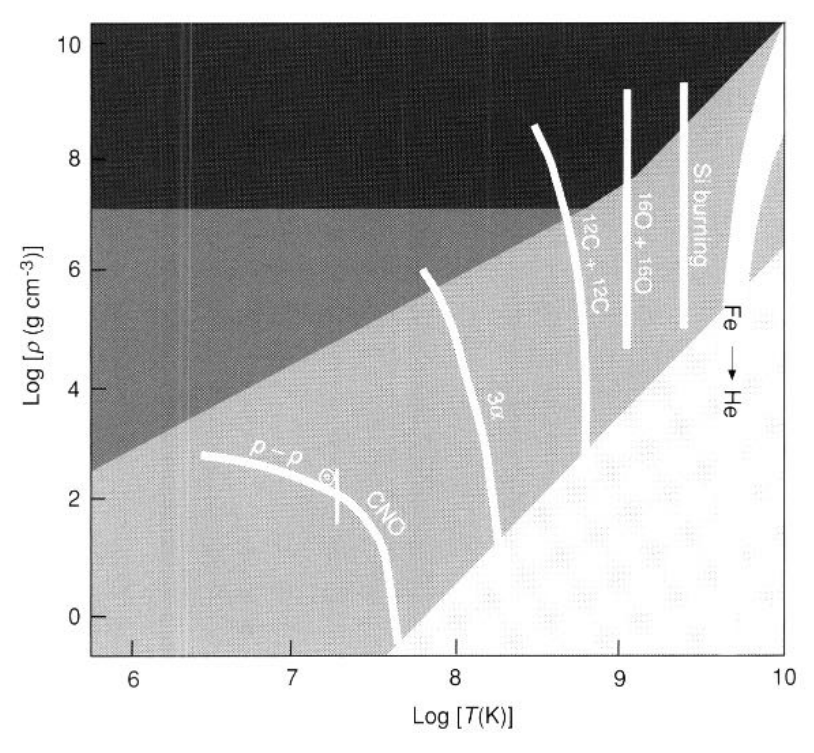
\includegraphics[width=6.5cm]{figures//Prialnik_logTlogrho_nuc.png}
\caption*{Credits: Prialnik}
\end{figure}
\end{minipage}
}
%
%
\frame{
\frametitle{Zones of nuclear burning}
\begin{minipage}{0.5\linewidth}
\begin{itemize}
\item The Hydrogen burning reactions connect smoothly from the $pp$
  chain to the CNO cycle. The latter has much stronger $T$-dependence
  and hence the slope in the ($T,\rho$) plane is steeper.
\item Further reactions include helium, carbon, oxygen, and silicon
  burning, that are activated at higher $T$.
\item For $T$ reaching several billion Kelvin, iron cores start to
  dissociate which plays role at late stages of massive stars.
\end{itemize}
\end{minipage}
\begin{minipage}{0.49\linewidth}
\begin{figure}
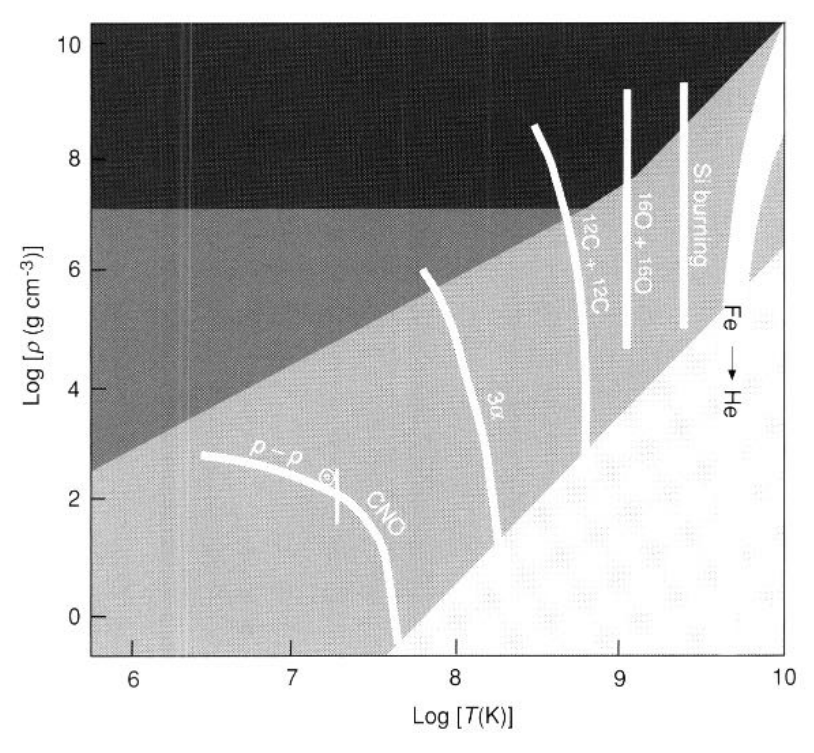
\includegraphics[width=6.5cm]{figures//Prialnik_logTlogrho_nuc.png}
\caption*{Credits: Prialnik}
\end{figure}
\end{minipage}
}
%
%
\frame{
\frametitle{A note on dynamical stability}
\begin{itemize}
\item Consider a macroscopic radial perturbation in a gas sphere of
  mass $M$ in hydrostatic equilibrium. Pressure at any point is the
  weight per unit area between layers $m$ and $M$:
  \begin{equation}
    p = \int_m^M \frac{Gm}{4\pi r^4} dm.
  \end{equation}
  The density is given by
  \begin{equation}
    \rho = \frac{1}{4\pi r^2} \frac{dm}{dr}.
  \end{equation}
\item Consider a small radial compression such that the radii are
  obtained from
  \begin{equation}
    r' = r - \epsilon r = r(1 - \epsilon).
  \end{equation}
\item For $\epsilon \ll 1$ the binomial expansion gives:
  \begin{equation}
    (1 \pm \epsilon)^n \approx 1 \pm n\epsilon.
  \end{equation}
\end{itemize}
}
%
%
\frame{
\frametitle{A note on dynamical stability}
\begin{itemize}
\item Therefore the new density is:
  \begin{equation}
    \rho' = \frac{1}{4\pi r^2 (1-\epsilon)^2} \frac{dm}{dr}
    \frac{dr}{dr'} = \frac{\rho}{(1-\epsilon)^3} \approx
    \rho(1+3\epsilon).
  \end{equation}
\item Assume that the contraction is adiabatic, the perturbed pressure
  is related to the original one via $(\rho'/\rho)^\gamma$, where
  $\gamma$ is the adiabatic exponent. Thus,
  \begin{equation}
    \pgas' = p(1+3\epsilon)^\gamma \approx p(1+3\gamma\epsilon).\label{equ:pgasp}
  \end{equation}
\item The new hydrostatic pressure is
  \begin{equation}
    p'_h = \int_m^M \frac{Gm}{4\pi r^4 (1-\epsilon)^4} dm \approx p
    (1+4\epsilon).\label{equ:phyd}
  \end{equation}
\end{itemize}
}
%
%
\frame{
\frametitle{A note on dynamical stability}
\begin{itemize}
\item The gas sphere is no longer in hydrostatic equilibrium, i.e.,
  $\pgas' \neq p'_h$. Condition for restoring equilibrium is
  \begin{equation}
    \pgas' > p'_h,
  \end{equation}
  such that the sphere expands to it original state.
\item From Eqs.~(\ref{equ:pgasp}) and (\ref{equ:phyd}) we can write
  this as
  \begin{equation}
    p(1+3\gamma\epsilon) > p (1+4\epsilon).
  \end{equation}
\item From this we can read the condition for \emph{dynamical
stability}:
  \begin{equation}
    \gamma > \fourthirds.
  \end{equation}
\item If $\gamma < \fourthirds$ somewhere (but not throughout) the
  star, stability is determined by the integral
  \begin{equation}
    \int \left(\gamma - \fourthirds \right) \frac{p}{\rho} dm.
  \end{equation}
 Instability occurs if the integral is negative.
\end{itemize}
}
%
%
\frame{
\frametitle{A note on dynamical stability}
\begin{itemize}
\item For relativistic-degenerate electron gas $\gamma =
  \fourthirds$. This is the limiting case corresponding to the
  Chandrasekhar mass $M_{\rm Ch}\sim 1.46M_\odot$. If the mass is
  higher a perturbation leads to collapse of the star.
\item If radiation pressure becomes dominant such that $p\approx
%($\beta \rightarrow 0$)
  \prad$, $\gamma \rightarrow \fourthirds$.
\item For pure photon gas $p/\rho = u_{\rm rad}/3$. Using the virial
  theorem, we get
  \begin{equation}
    -\Omega = 3 \int_0^M \frac{p}{\rho}dM = u_{\rm rad}.
  \end{equation}
  This means that the total energy of the star $E = \Omega + u_{\rm
    rad}$ vanishes.
\item This means that the gas sphere is \emph{unbound}.
\end{itemize}
}
%
%
\frame{
\frametitle{A note on dynamical stability}
\begin{itemize}
\item An ionistation(-type) process can change the adiabatic index and
  lead to $\gamma < \fourthirds$.
\item The most obvious example is ionisation where a single atom can
  produce two particles if a suitable amount of energy is absorbed or
  via a collision with another particle or photon.
\item The reverse process (recombination) occurs at the same time and
  reduces the number of particles.
\item Because pressure depends on the number of particles irrespective
  of their nature, ionisation/recombination leads to a dependence of
  the pressure on volume (density) is different than for ideal gas.
\item As an example, for a pure singly ionized gas $\gamma <
  \fourthirds$ between 18\% and 82\% ionization. Therefore only a
  nearly neutral or nearly completely ionized gas would be dynamically
  stable.
\end{itemize}
}
%
%
\frame{
\frametitle{Zones of instability}
\begin{minipage}{0.5\linewidth}
\begin{itemize}
\item In regions III and IV $\gamma \rightarrow \fourthirds$ due to
  relativistic degenerate gas and radiation presure,
  respectively. Therefore dynamical instability can also occur.
\item Further regions where dynamical instability occurs include the
  iron photodisintegration zone and pair production strip which are
  ionization-like nuclear processes.
\item Therefore the stable part of the ($\rho,T$) diagram is bounded
  by high temperatures and high density regions.
\item Furthermore, nuclear burning is \emph{thermally} unstable in
  degenerate gases.
\end{itemize}
\end{minipage}
\begin{minipage}{0.49\linewidth}
\begin{figure}
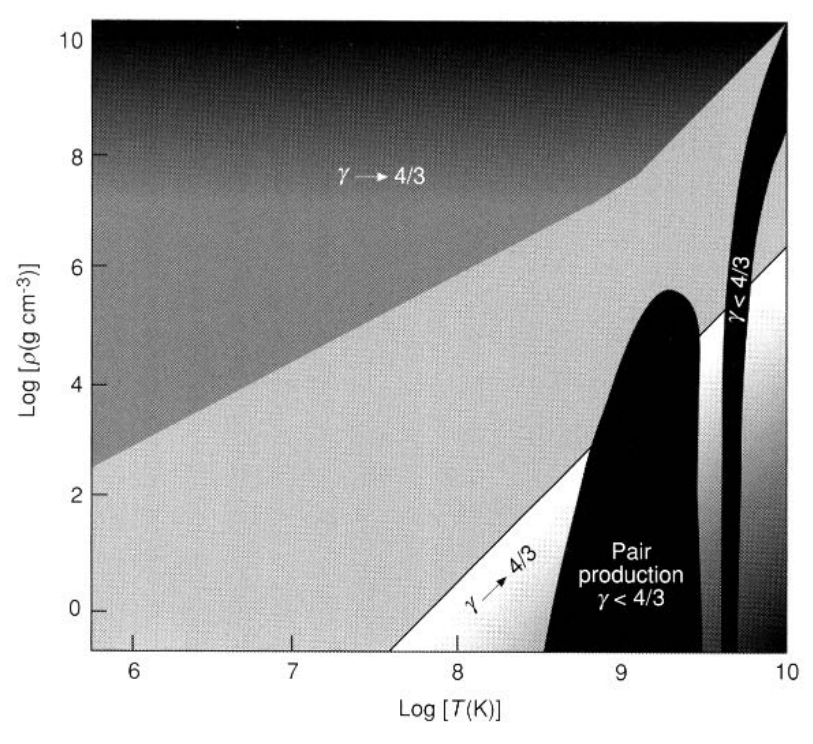
\includegraphics[width=6.5cm]{figures//Prialnik_logTlogrho_sta.png}
\caption*{Credits: Prialnik}
\end{figure}
\end{minipage}
}
%
%
\frame{
\frametitle{Evolutionary path of the centre of the star in the ($\log T, \log\rho$) plane}
\begin{minipage}{0.5\linewidth}
\begin{itemize}
\item Consider a polytropic configuration for a star in hydrostatic
  equilibrium. Then the central density is
  \begin{equation}
    p_{\rm c} = (4\pi)^{1/3} B_n G M ^{2/3} \rhoc^{4/3},\label{equ:pc}
  \end{equation}
  where the coefficient $B_n$ is a weak function of the polytropic
  index in the range $n = 1.5\ldots 3$.
\item Consider a star in zone I where ideal gas equation applies. Then
  the relation between $\rhoc$ and $\TTc$ is
  \begin{equation}
    \rhoc = \frac{K_0^3}{4\pi B_n^3 G^3} \frac{\TTc^3}{M^2}.
  \end{equation}
\end{itemize}
\end{minipage}
\begin{minipage}{0.49\linewidth}
\begin{figure}
\includegraphics[width=6.5cm]{figures//Prialnik_logTlogrho_rhocTc.png}
\caption*{Credits: Prialnik}
\end{figure}
\end{minipage}
}
%
%
\frame{
\frametitle{Evolutionary path of the centre of the star in the ($\log T, \log\rho$) plane}
\begin{minipage}{0.5\linewidth}
\begin{itemize}
\item For a given density the temperature increasea when the mass of
  the star increases. This leads to parallel lines whose intersections
  at a given $\rho$ differ by $\log M$.
\item If the gas at the centre is  degenerate, $\rhoc$ is given by
  \begin{equation}
    \rhoc = 4\pi \left(\frac{B_{1.5} G}{K_1} \right)^3 M^2.\label{equ:rhocp}
  \end{equation}
  These are horizontal lines in the ($\log T, \log\rho$)-plane. Note
  that $\rhoc$ is independent from $\TTc$.
\end{itemize}
\end{minipage}
\begin{minipage}{0.49\linewidth}
\begin{figure}
\includegraphics[width=6.5cm]{figures//Prialnik_logTlogrho_rhocTc.png}
\caption*{Credits: Prialnik}
\end{figure}
\end{minipage}
}
%
%
\frame{
\frametitle{Evolutionary path of the centre of the star in the ($\log T, \log\rho$) plane}
\begin{minipage}{0.5\linewidth}
\begin{itemize}
\item The density of degenerate stars tends to infinity as the stellar
  mass tends to the Chandrasekhar mass $M_{\rm Ch}$ (tutorials).
%\item This mass is obtained by equating Eq.~(\ref{equ:pc}) and
%  (\ref{equ:perdeg}).
  %% \begin{equation}
  %%   M^{-2/3} = (4\pi)^{1/3} B_n \frac{G}{K_1} 
  %% \end{equation}  
  %% \begin{equation}
  %%   M = ((4\pi)^{1/3})^{-3/2} \left(\frac{K_1} {B_n G} \right)^{3/2}
  %% \end{equation}  
\item This mass separates the regions I and III and the ``knee''
  curves for $M<M_{\rm Ch}$ and the straight ones for $M>M_{\rm Ch}$.
\end{itemize}
\end{minipage}
\begin{minipage}{0.49\linewidth}
\begin{figure}
\includegraphics[width=6.5cm]{figures/Prialnik_logTlogrho_rhocTc.png}
\caption*{Credits: Prialnik}
\end{figure}
\end{minipage}
}
%
%
\frame{
\frametitle{Evolutionary path of the centre of the star in the ($\log T, \log\rho$) plane}
\begin{minipage}{0.5\linewidth}
\begin{itemize}
\item Combination of all of the information so far can be used to
  sketch the evolutionary of stars with different masses.
\item This can be used to sketch the general paths of stars of
  different masses.
\item Stars have a minimum and maximum masses. \blue{Why?}
\end{itemize}
\end{minipage}
\begin{minipage}{0.49\linewidth}
\begin{figure}
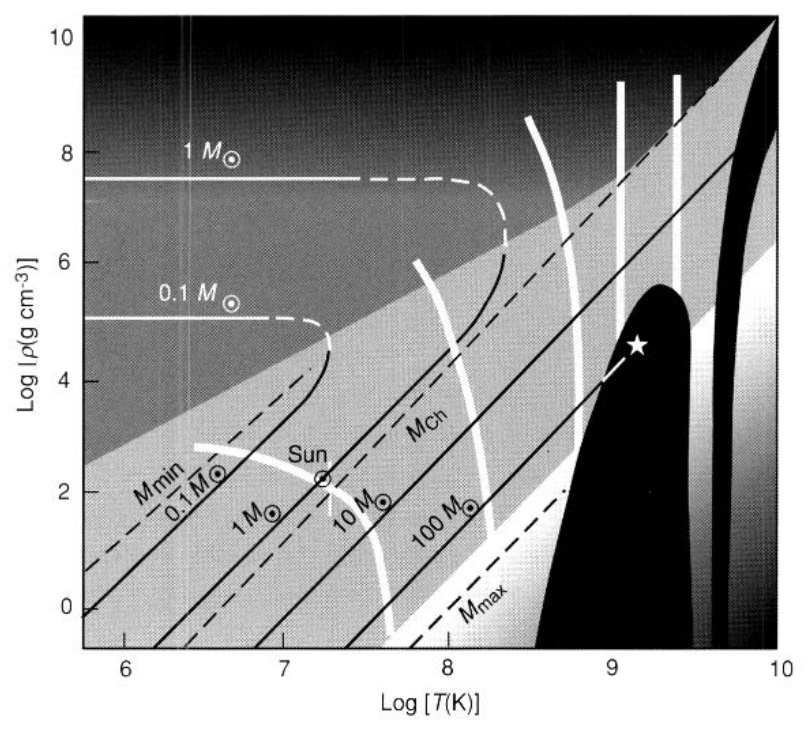
\includegraphics[width=6.5cm]{figures/Prialnik_logTlogrho_evo.png}
\caption*{Credits: Prialnik}
\end{figure}
\end{minipage}
}
%
%
\frame{
\frametitle{Evolutionary path of the centre of the star in the ($\log T, \log\rho$) plane}
\begin{minipage}{0.5\linewidth}
\begin{itemize}
\item Combination of all of the information so far can be used to
  sketch the evolutionary of stars with different masses.
\item This can be used to sketch the general paths of stars of
  different masses.
\item Stars have a minimum and maximum masses. \blue{Why?}
\item The cores of stars with $M \lesssim 0.08 M_\odot$ are not hot
  enouhg to ignite nuclear fusion. For $M \gtrsim100 M_\odot$ the
  radiation pressure makes the star unbound.
\end{itemize}
\end{minipage}
\begin{minipage}{0.49\linewidth}
\begin{figure}
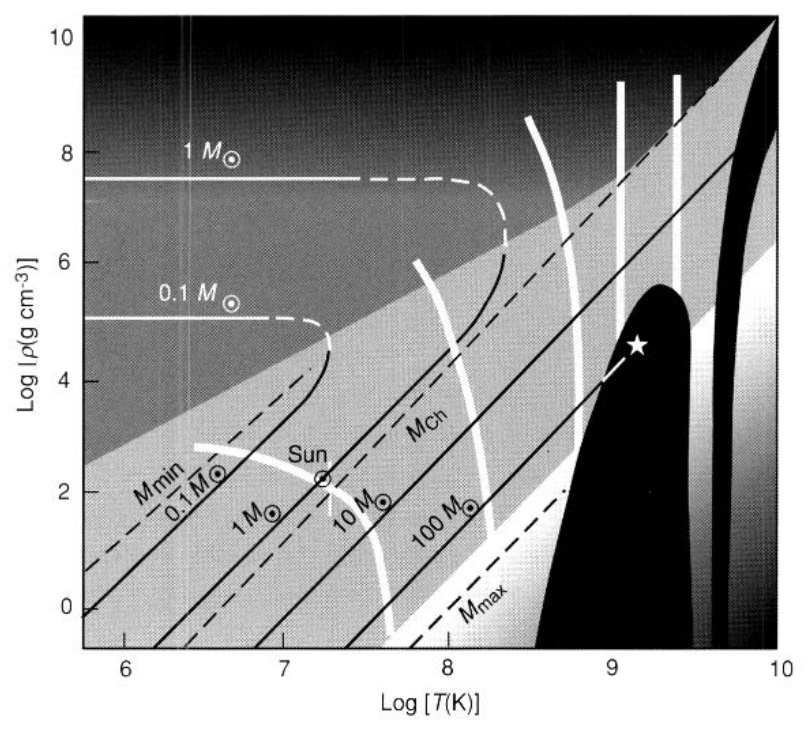
\includegraphics[width=6.5cm]{figures/Prialnik_logTlogrho_evo.png}
\caption*{Credits: Prialnik}
\end{figure}
\end{minipage}
}
%
%
\frame{
\frametitle{Evolutionary path of the centre of the star in the ($\log T, \log\rho$) plane}
\begin{minipage}{0.5\linewidth}
\begin{itemize}
\item Low mass stars contract and heat up until hydrogen burning
  commences. The stars remain in this evolutionary phase for a very
  long (nuclear) time.
\item When hydrogen is depleted from the core, degeneracy starts to
  play a role. Therefore stars with $M<M_{\rm Ch}$ end up as white
  dwarfs and cool over again a long time.
\item White dwarfs have a constant radius and density that depend only
  on the mass $M$. The larger the mass, the lower the radius.
\item We would expect two populations of white dwarfs. \blue{Why?}
\end{itemize}
\end{minipage}
\begin{minipage}{0.49\linewidth}
\begin{figure}
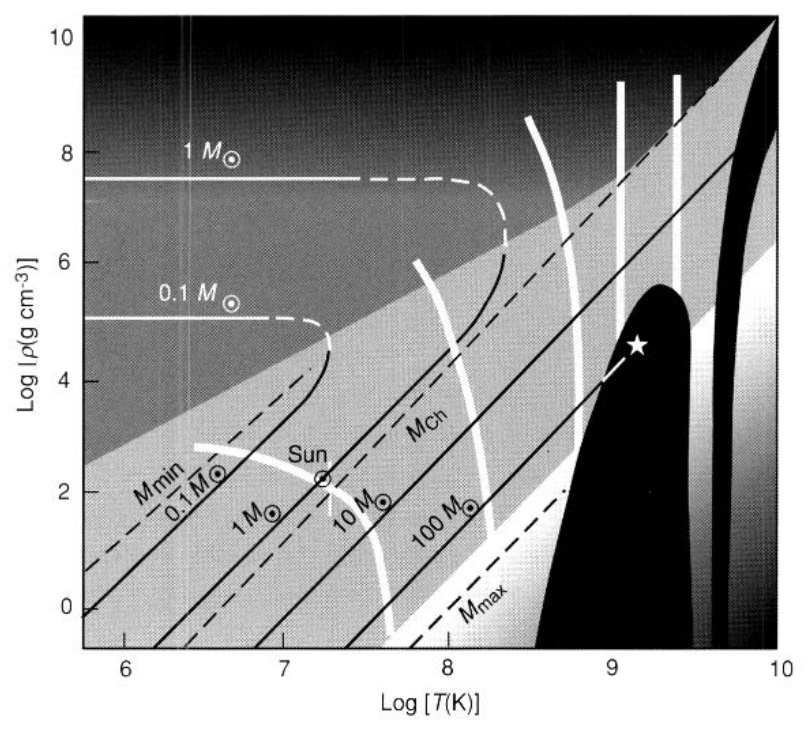
\includegraphics[width=6.5cm]{figures/Prialnik_logTlogrho_evo.png}
\caption*{Credits: Prialnik}
\end{figure}
\end{minipage}
}
%
%
\frame{
\frametitle{Evolutionary path of the centre of the star in the ($\log T, \log\rho$) plane}
\begin{minipage}{0.5\linewidth}
\begin{itemize}
\item Stars near $M=M_{\rm Ch}$ cross the carbon detonation very near
  the degeneracy border that can lead to a thermonuclear instability
  and collase. \blue{Why is this very unlikely for a single star?}
\item More massive stars burn successively heavier elements as the
  lighter ones have been consumed. Eventually they hit the iron
  photodissociation strip where another catastrophic instability
  happens.
\item The most massive stars can hit the pair-production instability
  strip even earlier than this.
\end{itemize}
\end{minipage}
\begin{minipage}{0.49\linewidth}
\begin{figure}
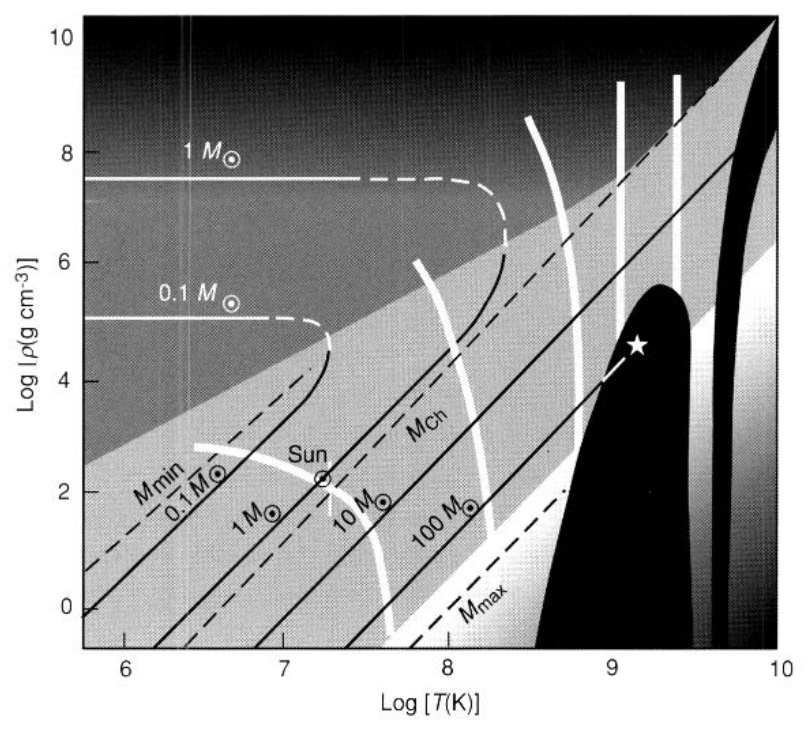
\includegraphics[width=6.5cm]{figures/Prialnik_logTlogrho_evo.png}
\caption*{Credits: Prialnik}
\end{figure}
\end{minipage}
}
%
%
\frame{
\frametitle{Theory of the main sequence}
\begin{minipage}{0.59\linewidth}
\begin{itemize}
\item There is an observed relation between the luminosity and
  effective temperature of main sequence stars
  \begin{equation}
    \log L = \alpha \log \Teff + {\rm const.},\label{equ:logL}
  \end{equation}
  where the slope $\alpha$ is different for low and large $L$.
\item Another apparent correlation exists between luminosity and mass:
  \begin{equation}
    L \propto M^\nu.\label{equ:Lmass}
  \end{equation}
\item Based on our theory, we make a hypothesis that main sequence
  stars burn hydrogen in their cores and are correspondingly placed on
  the ($\log T, \log \rho$) plane. This theory needs to reproduce the
  relations (\ref{equ:logL}) and (\ref{equ:Lmass}).
\end{itemize}
\end{minipage}
\begin{minipage}{0.4\linewidth}
\begin{figure}
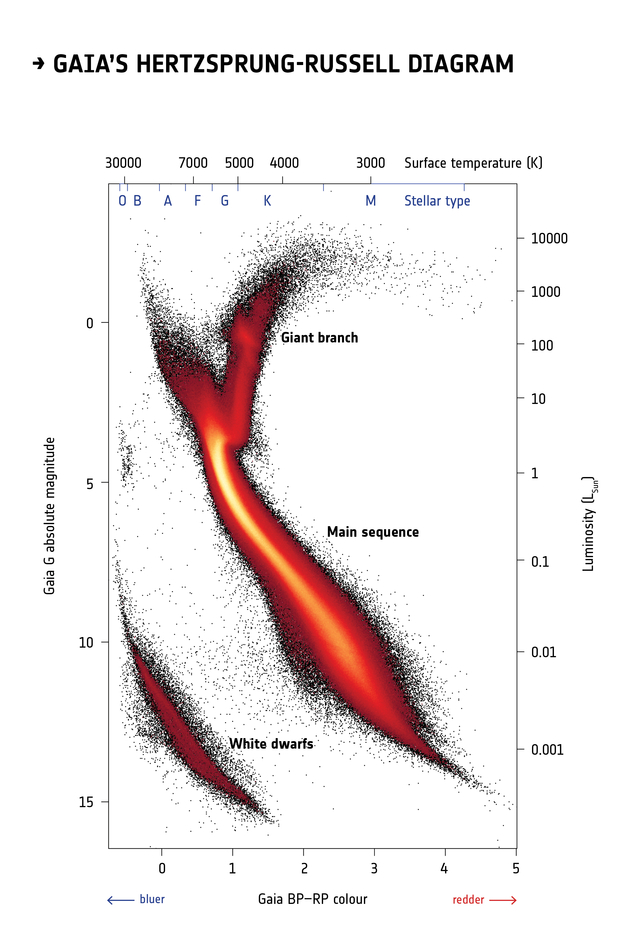
\includegraphics[width=5cm]{figures/Gaia_HR.jpg}
\caption*{Credits: ESA}
\end{figure}
\end{minipage}
}
%
%
\frame{
\frametitle{Theory of the main sequence}
\begin{itemize}
\item Assume stars that have started to burn hydrogen at the centre
  and are in thermal and hydrostatic equilibrium. We assume uniform
  chemical composition, radiative equilibrium, neglect radiation
  pressure and assume analytic (constant) opacity.
\item Now the governing equations are:
  \begin{eqnarray}
    \frac{dp}{dm} &=& - \frac{Gm}{4\pi r^4},\ \ \ \frac{dr}{dm} = \frac{1}{4\pi r^2 \rho}, \\
    \frac{dT}{dm} &=& - \frac{3}{4ac} \frac{\kappa}{T^3} \frac{F}{(4\pi r^2)^2}, \ \ \ \frac{dF}{dm} = q_o \rho T^n,\ \ \ p = \frac{\cal R}{\mu} \rho T.
  \end{eqnarray}
\item This set of equations needs to be solved for $r(m)$, $p(m)$,
  $T(m)$, and $F(m)$ in the range $0 \leq m \leq M$ for any valu of
  $M$ which is a free parameter.
\item We would want to get some insight without actually solving the
  equations. \blue{How?}
\end{itemize}
}
%
%
\frame{
\frametitle{Theory of the main sequence}
\begin{itemize}
\item The answer is \emph{dimensional analysis} that we already used
  on some of the tutorials.
\item Let us first define a dimensionless variable for the fractional mass:
  \begin{equation}
    x = \frac{m}{M}.
  \end{equation}
\item The functions $r(m)$, $p(m)$, $T(m)$, and $F(m)$ can then be
  replaced by non-dimensional functions that depend on $x$: $f_1(x)$,
  $f_2(x)$, $f_3(x)$, etc.
\item We end up with:
  \begin{eqnarray}
    r = f_1(x) \Rstar,\ \ p = f_2(x) \pstar,\ \ \rho = f_3(x) \rhostar,\ \ T = f_4(x) \Tstar,\ \ F = f_5(x) \Fstar, \label{equ:nondim}
  \end{eqnarray}
  where the starred quantities have the dimensions of the original
  functions.
\end{itemize}
}
%
%
\frame{
\frametitle{Theory of the main sequence}
\begin{itemize}
\item As an example, substituting the relations $r = f_1(x) \Rstar$,
  $p = f_2(x) \pstar$, and $\rho = f_3(x) \rhostar$ into equation
  of hydrostatic equilibrium yields
  \begin{equation}
    \frac{\pstar}{M} \frac{df_2}{dx} = - \frac{GMx}{4\pi f_1^4 \Rstar^4}.
  \end{equation}
\item Since the units of both sides must match and $f_i$ are
  non-dimensional, $\pstar$ must be proportional to $GM^2/\Rstar^4$.
\item Setting the coefficient of proportionality to unity leads to:
  \begin{equation}
    \frac{df_2}{dx} = - \frac{x}{4\pi f_1^4},\ \ \ \pstar = \frac{GM^2}{\Rstar^4}.
  \end{equation}
\end{itemize}
}
%
%
\frame{
\frametitle{Theory of the main sequence}
\begin{itemize}
\item Repeating the exercise for the other four equations:
  \begin{equation}
    \begin{split}
      \frac{df_1}{dx} &= \frac{1}{4\pi f_1^2 f_3},\\
                  f_2 &= f_3 f_4,\\
      \frac{df_4}{dx} &= - \frac{3f_5}{4f_4^3(4\pi f_1^2)^2},\\
      \frac{df_5}{dx} &= f_3 f_4^n,\\
    \end{split}
    \hspace{2cm}
    \begin{split}
     \rhostar &= \frac{M}{\Rstar^3}, \\
     \Tstar &= \frac{\mu \pstar}{{\cal R} \rhostar}, \\
     \Fstar &= \frac{ac}{\kappa} \frac{\Tstar^4 \Rstar^4}{M}, \\
     \Fstar &= q_0 \rhostar \Tstar^n M. \label{equ:stars}
    \end{split}
  \end{equation}
\item The equations on the lhs are non-linear differential equations
  for $f_i$ in the range $0 \leq x \leq 1$. The dimensional quantities
  on the rhs of Eq.~(\ref{equ:nondim}) are obtained from the
  \emph{algebraic} Eqs.~(\ref{equ:stars}) (right).
\item Combination of these differential and algebraic equations allows
  for solving the interior structure for any mass $M$. Importantly the
  profiles as function of $x$ are the same in all stars, differing
  only by a constant factor determined by the mass. This property is
  called \emph{homology}.
\end{itemize}
}
%
%
\frame{
\frametitle{Theory of the main sequence}
\begin{itemize}
\item Now we can skip solving the differential equations if we are
  just interested in the dependence of physical properties on $M$.
\item Solving for $\Tstar$ gives:
  \begin{equation}
    \Tstar = \frac{\mu G}{\cal R}\frac{M}{\Rstar}.
  \end{equation}
  Using this in the first equation for $\Fstar$ gives:
  \begin{equation}
    \Fstar = \frac{ac}{\kappa} \left( \frac{\mu G}{\cal R} \right)^4 M^3.
  \end{equation}
\item Since this relation is valid for any value of $x$, the surface
  value scales as
  \begin{equation}
    L \propto M^3,
  \end{equation}
  which can be compared with observations.
\end{itemize}
}
%
%
\frame{
\frametitle{Theory of the main sequence}
\begin{itemize}
\item Furthermore, we can now solve for (exercises) $\Rstar$ and
  $\rhostar$:
  \begin{equation}
    \Rstar \propto M^{\frac{n-1}{n+3}},\ \ \ \rhostar \propto M^{2\frac{3-n}{3+n}}.
  \end{equation}
  \blue{What can be concluded based on these relations?}
\end{itemize}
}
%
%
\frame{
\frametitle{Theory of the main sequence}
\begin{itemize}
\item Furthermore, we can now solve for (exercises) $\Rstar$ and
  $\rhostar$:
  \begin{equation}
    \Rstar \propto M^{\frac{n-1}{n+3}},\ \ \ \rhostar \propto M^{2\frac{3-n}{3+n}}.
  \end{equation}
  \blue{What can be concluded based on these relations?}
\item $n\approx 16$ for the CNO cycle so stellar radius is almost
  independent of mass. For $pp$ chain $n\approx 4$ and $\Rstar \propto
  M^{3/7}$. Radius always increases with mass unlike for white dwarfs!
\item Since $n>3$, density decreases with increasing $M$ again
  opposite to white dwarfs.
\end{itemize}
}
%
%
\frame{
\frametitle{Theory of the main sequence}
\begin{itemize}
\item We are now in a position to compare with the observed HR
  diagram. The relation between luminosity and effective temperature
  is given by:
  \begin{equation}
    L = 4\pi R^2 \sigma \Teff^4.
  \end{equation}
\item Using the mass-luminosity and mass-radius relations to eliminate
  $\Rstar$ and $M$, we arrive at
  \begin{equation}
    L^{1 - \frac{2(n-1)}{3(n+3)}} \propto \Teff^4.
  \end{equation}
\item For $n=4$ this yields
  \begin{equation}
    \log L = 5.6\log \Teff + {\rm const.},
  \end{equation}
  and for $n=16$ we get
  \begin{equation}
    \log L = 8.4\log \Teff + {\rm const.}
  \end{equation}
\item These match with the observations fairly well.
\end{itemize}
}
%
%
%% \frame{
%% \frametitle{Evolutionary phases of a $10M_\odot$ star}
%% \begin{minipage}{0.5\linewidth}
%% \begin{itemize}
%% \item TBA
%% \end{itemize}
%% \end{minipage}
%% \begin{minipage}{0.49\linewidth}
%% \begin{figure}
%% 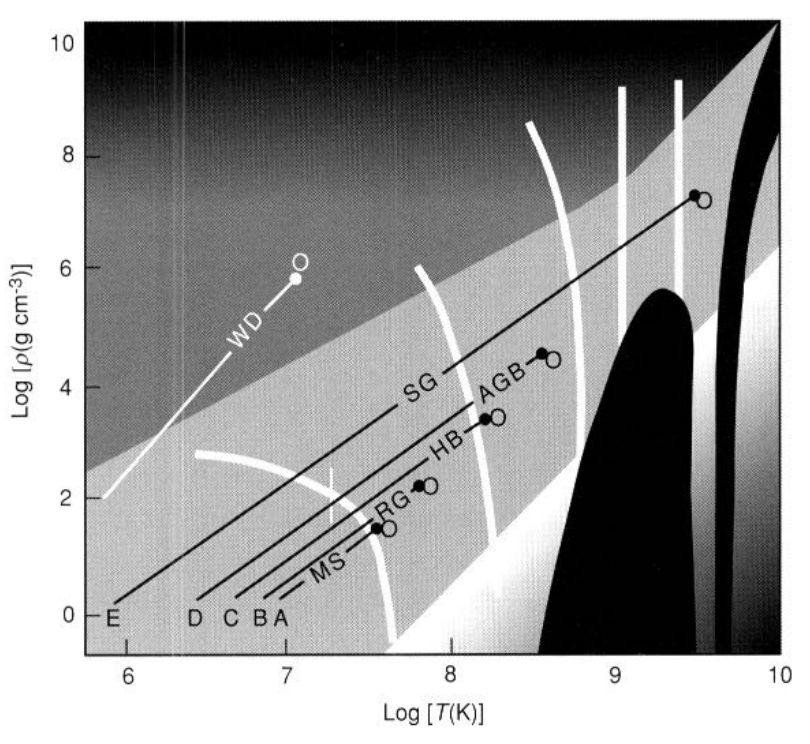
\includegraphics[width=6.5cm]{figures//Prialnik_logTlogrho_evo2.png}
%% \caption*{Credits: Prialnik}
%% \end{figure}
%% \end{minipage}
%%}
%
%
\frame{
\frametitle{Limitations of the simple model}
\begin{minipage}{0.5\linewidth}
\begin{itemize}
\item TBA
\end{itemize}
\end{minipage}
\begin{minipage}{0.49\linewidth}
\begin{figure}
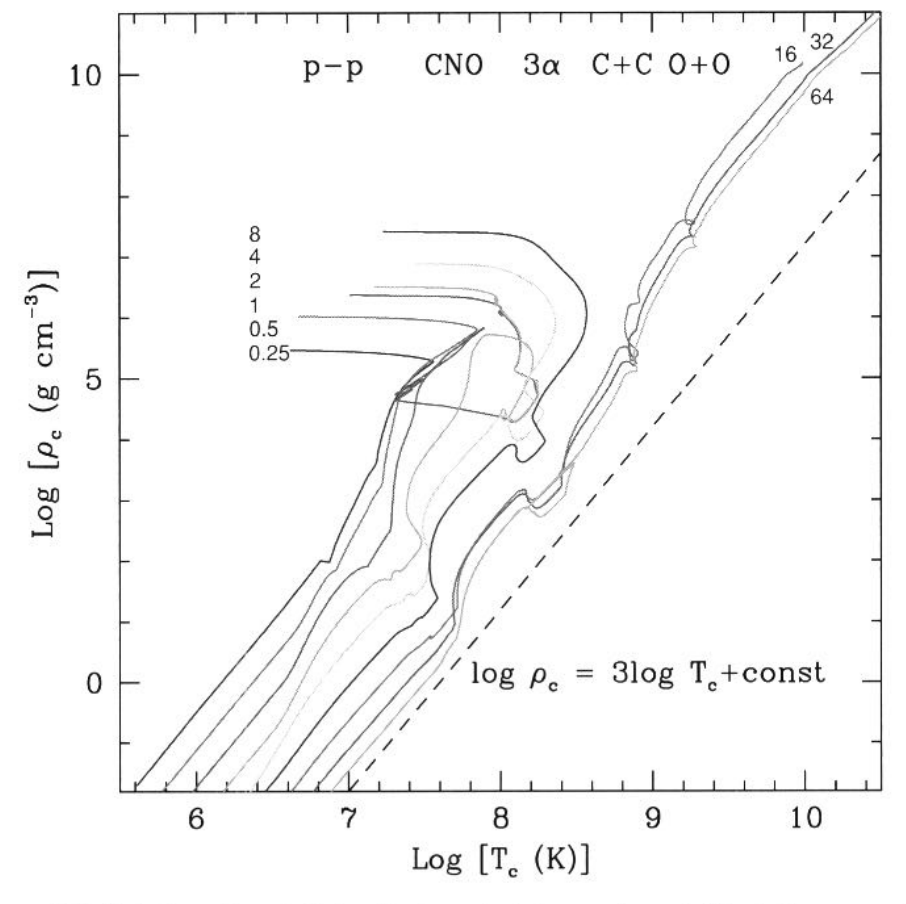
\includegraphics[width=6.5cm]{figures//Prialnik_logTlogrho_evoreal.png}
\caption*{Credits: Prialnik}
\end{figure}
\end{minipage}
}
%
%
\end{document}
% 

